\documentclass[10pt]{beamer}

\usetheme[progressbar=frametitle]{metropolis}
\usepackage{appendixnumberbeamer}

\usepackage{booktabs}
\usepackage[scale=2]{ccicons}

\usepackage{pgfplots}
\usepgfplotslibrary{dateplot}

\usepackage{xspace}
\newcommand{\themename}{\textbf{\textsc{metropolis}}\xspace}

\title{Tecniche di animazione 3D nella realizzazione di un cortometraggio}
\subtitle{}
% \date{\today}
\date{10 Dicembre 2019}
\author{Leonardo Marini}
\institute{ALMA MATER STUDIORUM - UNIVERSITÀ DI BOLOGNA}
%\titlegraphic{\hfill
\includegraphics[height=1.5cm]{logo.pdf}}

\begin{document}

\maketitle

\begin{frame}{Table of contents}
  \setbeamertemplate{section in toc}[sections numbered]
  \tableofcontents%[hideallsubsections]
\end{frame}

\section[Intro]{Introduzione}
% L'oggetto della mia tesi è la realizzare un cortometraggio con l'uso della computer grafica e, nella sua progettazione, analizzare le tecniche di animazione 3D che vengono solitamente usate.

\begin{frame}[fragile]{La storia}
  \begin{columns}[T,onlytextwidth]
    \column{0.33\textwidth}
      \begin{figure}
          \centering
          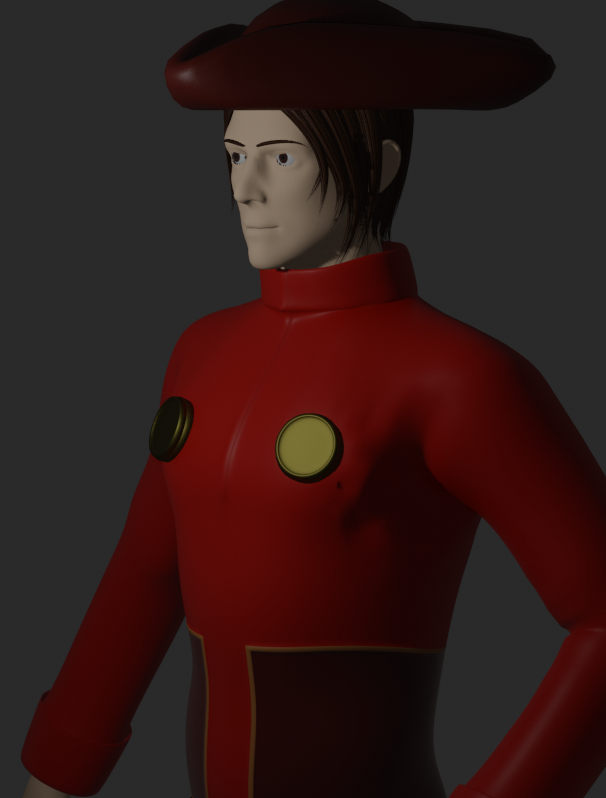
\includegraphics[width=\textwidth]{figures/Capitano.png}
          \caption{Capitano}
      \end{figure}

    \column{0.33\textwidth}
      \begin{figure}
          \centering
          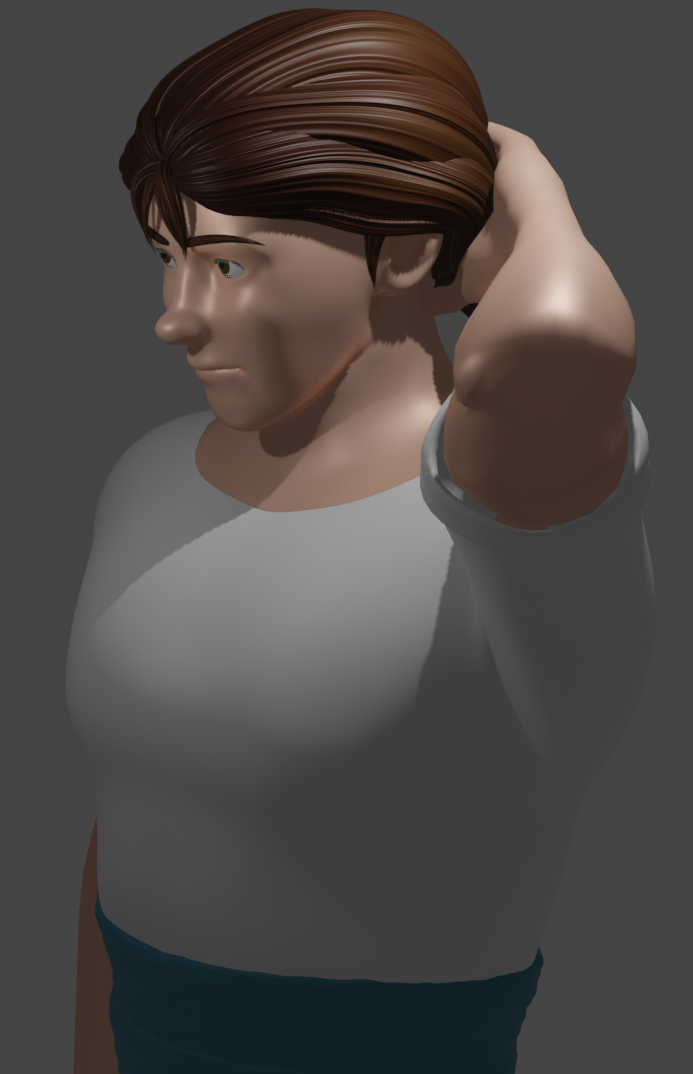
\includegraphics[width=\textwidth]{figures/ragazzo.png}
          \caption{Ragazzo}
      \end{figure}

    \column{0.33\textwidth}
      \begin{figure}
          \centering
          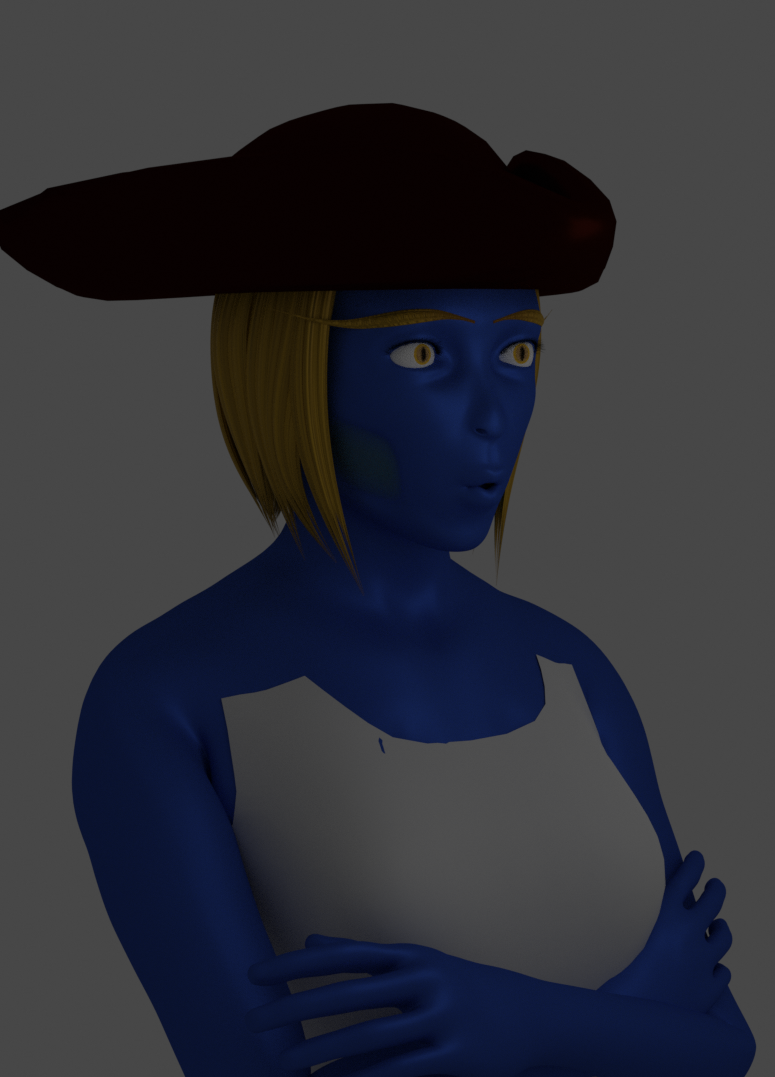
\includegraphics[width=\textwidth]{figures/Capitana.png}
          \caption{Capitana}
      \end{figure}
  \end{columns}
\end{frame}

\begin{frame}{Analisi}
\end{frame}

\section{Concetti di animazione}
\begin{frame}{Rappresentazioni di rotazione}
  \begin{columns}[T,onlytextwidth]
    \column{0.33\textwidth}
    Euler
      \begin{itemize}[<+- | alert@+>]
        \item Conceptually simple
        \item Complex and confusing in practice
        \item Multiple rotation order
        \item Gimbal lock and weird interpolation
      \end{itemize}

    \column{0.33\textwidth}
      Quaternions
      \begin{itemize}[<+- | alert@+>]
        \item No gimbal lock/changing axes
        \item Interpolation is smooth and direct
        \item Simple to do calculations with
        \item Consistent and predictable interpolation
      \end{itemize}
      
    \column{0.33\textwidth}
    Matrici
      \begin{itemize}[<+- | alert@+>]
        \item \alert<5>{Qualsiasi tipo di trasformazione}
        \item Parenting
        \item Constraints
        \item Armature deform
      \end{itemize}
  \end{columns}
\end{frame}
\begin{frame}{FK}
\end{frame}
\begin{frame}{IK}
\end{frame}

\section{Progettazione}
\begin{frame}{Generale}
\end{frame}
\begin{frame}{Animazioni/Rigging}
\end{frame}

\section{Produzione}
\begin{frame}{Modellazione}
\end{frame}
\begin{frame}{Animazione}
\end{frame}

{\setbeamercolor{palette primary}{fg=orange}
\begin{frame}[standout]

Domande?

\end{frame}
}

\end{document}
